\documentclass[draft]{agujournal2019}
\usepackage{url} %this package should fix any errors with URLs in refs.
\usepackage{lineno}
\usepackage[inline]{trackchanges} %for better track changes. finalnew option will compile document with changes incorporated.
\usepackage{soul}
\linenumbers

\draftfalse

%% Enter journal name below.
%% Choose from this list of Journals:
%
% JGR: Atmospheres
% JGR: Biogeosciences
% JGR: Earth Surface
% JGR: Oceans
% JGR: Planets
% JGR: Solid Earth
% JGR: Space Physics
% Global Biogeochemical Cycles
% Geophysical Research Letters
% Paleoceanography and Paleoclimatology
% Radio Science
% Reviews of Geophysics
% Tectonics
% Space Weather
% Water Resources Research
% Geochemistry, Geophysics, Geosystems
% Journal of Advances in Modeling Earth Systems (JAMES)
% Earth's Future
% Earth and Space Science
% Geohealth
%


\journalname{JGR: Solid Earth}


\begin{document}

\title{High geomagnetic field intensity in the late Mesoproterozoic recorded by Midcontinent Rift anorthosite xenoliths}


\authors{Yiming Zhang\affil{1}, Nicholas L. Swanson-Hysell\affil{1}, Margaret S. Avery\affil{1,3}}

\affiliation{1}{Department of Earth and Planetary Science, University of California, Berkeley, CA, USA}
\affiliation{2}{Department of Earth and Environmental Sciences, University of Minnesota, Duluth, MN, USA}
\affiliation{3}{Geology, Minerals, Energy, and Geophysics Science Center, U.S. Geological Survey, Moffett Field, CA, USA}
\correspondingauthor{Yiming Zhang}{yimingzhang@berkeley.edu}


\begin{keypoints}
\item New ca. 1092 Ma Midcontinent Rift anorthosite record high paleointensity values
\item High VADM of the geomagnetic field is inconsistent with previous interpretation of Proterozoic long term decay
\item A strong geodynamo like today likely persisted for about 25 myr during the Midcontinent Rift development
\end{keypoints}


% keywords: absolute paleointensity, Laurentia, Midcontinent Rift, anorthosite, geodynamo



\begin{abstract}
New high-quality absolute paleointensity data from anorthosite xenoliths within the Beaver River diabase intrusions of the North American Midcontinent Rift (MCR) record an average virtual axial dipole moment (VADM) estimate of $\sim$80 ZAm$^2$ \textit{ca.} 1092 Ma. This cooling rate corrected paleointensity estimate from the MCR intrusive unit is similar to previous results from extrusive units that are dated to be \textit{ca.} 1108 Ma and \textit{ca.} 1085 Ma. Rock magnetic analyses and magnetic imaging reveal that the anorthosites can have abundant single-domain magnetic carriers that are ideal for paleointensity experiment, leading to a high success rate passing our selection criteria. Taken together, new and previously published paleointensity data from the Midcontinent Rift support that a geomagnetic field strength persisted through the Midcontinent Rift development and the data are inconsistent with the interpretation of a decay of Earth's geodynamo strength through the late Mesoproterozoic. 


\end{abstract}

\section*{Introduction}
%The question of the core and the importance of the observational data as complementary for numerical simulation work.

That we have a solid inner core today is the result of secular cooling and differentiation of the layered Earth. The timing of inner core formation during Earth's thermal evolution is amongst the major unsolved questions in Earth's history. Due to the uncertain constraints on the thermal conductivity of the core \cite{Konopkova2016a, Gomi2013a, Ohta2016a}, numerical simulations have given drastically different predictions on the inner core nucleation age, ranging from about half a billion years ago to prior to the Archean \cite{Pozzo2012a, Gubbins2004a, Nimmo2015a}. Some models have suggested the thermal convection dominated liquid core motion experienced a long-term waning before the onset of the nucleation of the inner core, which kick-started the rigorous compositional convection between the solid inner core and liquid outer core \cite<e.g>{Davies2021a}. A corollary of such a prediction is that the geomagnetic axial dipole field, which is generated by the fluid motion in the liquid core, would have been decaying before the emergence of the solid inner core, when a significant increase in Earth's axial dipole field strength occurred \cite{Aubert2009a, Davies2021a}. 

Paleomagnetic data from ancient rocks are one of the few types of observational data that bear on the long-term evolution of Earth’s core and can be used to test the predictions from numerical simulations. Paleointensity studies have found very low axial dipole moment (VDM) estimates from rocks formed in the late Ediacaran \cite{Bono2019a, Shcherbakova2019a, Thallner2021b}, followed by a recovery of strength near the  Ediacaran-Cambrian boundary. Other studies focusing on paleomagnetic directions have also found that the late Ediacaran might have been a period of time when the geomagnetic field were experiencing frequent reversals and waning of dipole dominance. It has been interpreted that these findings are consistent with the results of previous geodynamo models using high core conductivity values that suggest the inner core nucleation age being near the Ediacaran-Cambrian boundary. \citeA{Bono2019a} filtered previous data compiled within the PINT database based on a set of quality criteria. A polynomial fit through the resulting paleointensity compilation from the Archean and the Proterozoic was used to interpret that a decrease trend of the estimated geomagnetic dipole strength persisted through the Proterozoic. In addition, \citeA{Bono2019a} recovered very low paleointensity values from ca. 565 Ma single silicate crystals that were interpreted to be consistent with it reflecting the weak geodynamo near the Ediacaran-Cambrian boundary due to progressive cooling of the core before the onset of the rigorous compositional convection driven by the nucleation of the solid inner core. Such decay trend in the Neoproterozoic is recently supported by new low paleointensity estimates derived from the ca. 720 Ma Franklin Large Igneous Province \cite{Lloyd2021a}. 

However, previous paleointensity data from intrusive and extrusive rock units in the Mesoproterozoic Midcontinent Rift \cite{Pesonen1983a, Kulakov2013a, Sprain2018a} record Earth's virtual axial dipole moment (VADM) values similar to that of today and are inconsistent with the prediction of the long term decay curve (Fig. \ref{}). \citeA{Pesonen1983b} obtained an average virtual dipole moment of 93 ZAm$^2$ after applying a 13\% cooling rate correction (114 ZAm$^2$ before correction) using the ca. 1108 Ma Osler Volcanics, Maimainse Point volcanics, intrusive Logan Sills, Thunder Bay dikes, and the Baraga and Marquette dikes, as well as the ca. 1096 Ma North Shore Volcanic Group. \citeA{Sprain2018a} obtained more high-quality paleointensity data using the ca. 1108 Ma Osler Volcanics and the ca. 1100 Ma Mamainse Point volcanics. A calculated mean VADM value of 56 $\pm$ 21 ZAm$^2$ is similar to the average value of the past 300 million years. In addition, an average VADM of 59 $\pm$ 11 ZAm$^2$ obtained \citeA{Kulakov2013a} using the ca. 1085 Ma Lake Shore Traps volcanics suggests that the present-day-like geomagnetic field strength likely persisted through the late stage of Midcontinent Rift magmatism. Taken together, these rock units that have been dated to span $\sim$25 myr during the development of the Midcontinent Rift magmatism \cite{Swanson-Hysell2019a} may be incompatible with the hypothesis of a ``Proterozoic dipole low" \cite{Biggin2009a}. 

But the non-ideal paleointensity behaviors at specimen level and overall low success rates have challenged the interpretation of many previous paleointensity results. One typical failure of paleointensity experiment is the double-slope behavior, as two distinct paleointensity estimates may be calculated depending on the interpreter's choice of slope: a higher paleointensity estimate from the low-temperature portion and a lower paleointensity estimate from the high-temperature portion. \citeA{Pesonen1983a} used the low-temperature slope as the best representation of the past magnetic field strength whereas \citeA{Kulakov2013a} used the high-temperature slop. Such non-ideal behavior were interpreted as failure by \siteA{Sprain2018a} who applied stricter paleointensity selection criteria and accepted only 23 out of 133 specimens (5 out of 21 lava flows) from the Osler Volcanics and the Mamainse Point volcanics. Similar concern on paleointensity result quality led \citeA{Bono2019a} to exclude all paleointensity records from the Midcontinent Rift but those from \citeA{Kulakov2013a}. Nevertheless, specimens that yield dominantly single-slope paleointensity results from the ca. 1105 Ma Osler Volcanic Group, Mamainse Point volcanics \cite{Sprain2018a}, as well as the ca. 1085 Ma Lake Shore Traps \cite{Kulakov2013a} suggest VADM values similar to that of the present-day values \cite{Sprain2018a}, inconsistent with the interpretation of a low geomagnetic field strength during the Midcontinent Rift (Fig. \ref{}). 

Although it is typical of paleointensity experiments to suffer from low success rates, quenched volcanic glass \cite{Tauxe2004a} and single silicate minerals \cite{Tarduno2005a} are found to be able to produce high success rates, likely due to the magnetic carriers being dominated by single-domain magnetite and being well shielded by their host against thermochemical alteration during paleointensity experiments. In this study, we present new paleointensity results from ``IZZI" absolute paleointensity experiments \cite{Yu2004a} on a suite of ca. 1092 Ma anorthosite xenoliths and their diabase host rocks of the Beaver Bay Complex within the Midcontinent Rift. The anorthosite lithology yielded exceptionally high success rate thanks to the plagioclase crystals shielding the magnetic minerals within. With more single-slope, high quality paleointensity data we seek to compare paleointensity records from the Midcontinent Rift intrusives with those from the extrusives; to test the hypothesis that the Earth's geomagnetic dipole strength remained at high values throughout the Midcontinent Rift; and to further enrich the reliable paleointensity records during the $\sim$25 myr of Midcontinent Rift magmatic activity. 



%Retrieving paleomagnetic information from Precambrian rocks can aid in our understanding of the long-term evolution of the geodynamo. A recent paleointensity study by \cite{Sprain2018a} reported a ca. 1.1 Ga paleomagnetic field strength similar to today based on the volcanics of the Midcontinent Rift System (MRS). That study suggested that this result is consistent with models wherein this time period of the Proterozoic is characterized by a strong rather than weak geomagnetic field. However, to further evaluating the evolution of the geomagnetic field during the Precambrian, more paleointensity data are needed. 

%The MRS emplaced a vast amount of extrusive and intrusive rocks spanning a prolonged period of $\sim$25 Myrs. \cite{Swanson-Hysell2019a} published an extensive compilation of the MRS volcanics with paired high-precision CA-ID-TIMS U-Pb geochronology and high-quality paleomagnetic directions, revealing at least two dipole reversals and rapid differential plate motion of the ancient North American plate, Laurentia, during the emplacement of MRS. The synthesized North American apparent polar wander path (APWP) was interpreted to be composed primarily of rapid plate motion \citep{Swanson-Hysell2019a}. Through comparison between paleomagnetic pole positions and the APWP, such rapid plate motion and high-precision paleomagnetic and geochronological framework revealed by the MRS volcanics can provide insights into age constraints on units with poor or no geochronology data. This framework allows for further paleomagnetic contributions beyond the Midcontinent Rift volcanics. 

\section*{Geologic Settings}
% a map of the lake superior including the pesonen units, the lake shore traps, the BRD, and the osler and mamainse, together with date compilation. 

The North American Midcontinent Rift (MCR) is a failed intracontinental rift where protracted magmatic activity lasted from \textit{ca.} 1109 Ma to \textit{ca.} 1084 Ma \cite{Swanson-Hysell2019a}. Previous studies have divided magmatic activity in the rift into four stages based on interpreted changes in relative magmatic volume and the nature of magmatism: early ($\sim$1109–1104 Ma), latent ($\sim$1104–1098 Ma), main ($\sim$1098–1090 Ma) and late ($\sim$1090–1084 Ma) \cite{Vervoort2007a, Heaman2007a, Miller2013a}. In particular, the main stage magmatism is characterized by rapid and punctuated events which resulted in voluminous emplacement of intrusives as well as coeval outpouring of extrusives, as can be exampled by the massive ca. 1096 Ma Duluth Complex and the North Shore Volcanic Group \cite{Swanson-Hysell2020a}, the ca. 1092 Ma Beaver Bay Complex and the Portage Lake Volcanics (Fig. \ref{}; \citeA{Zhang2021a}. Excellent rock preservation thanks to minimal post-rift alteration in the Midcontinent Rift have yielded high-quality paleomagnetic directional data which have now been paired with high-precision zircon geochronology to reconstruct the well-resolved apparent polar wander path for Laurentia (cratonic North America) called the Keweenawan Track (Fig. \ref{}; \citeA{Swanson-Hysell2019a}). 

\begin{figure}
\centering
\noindent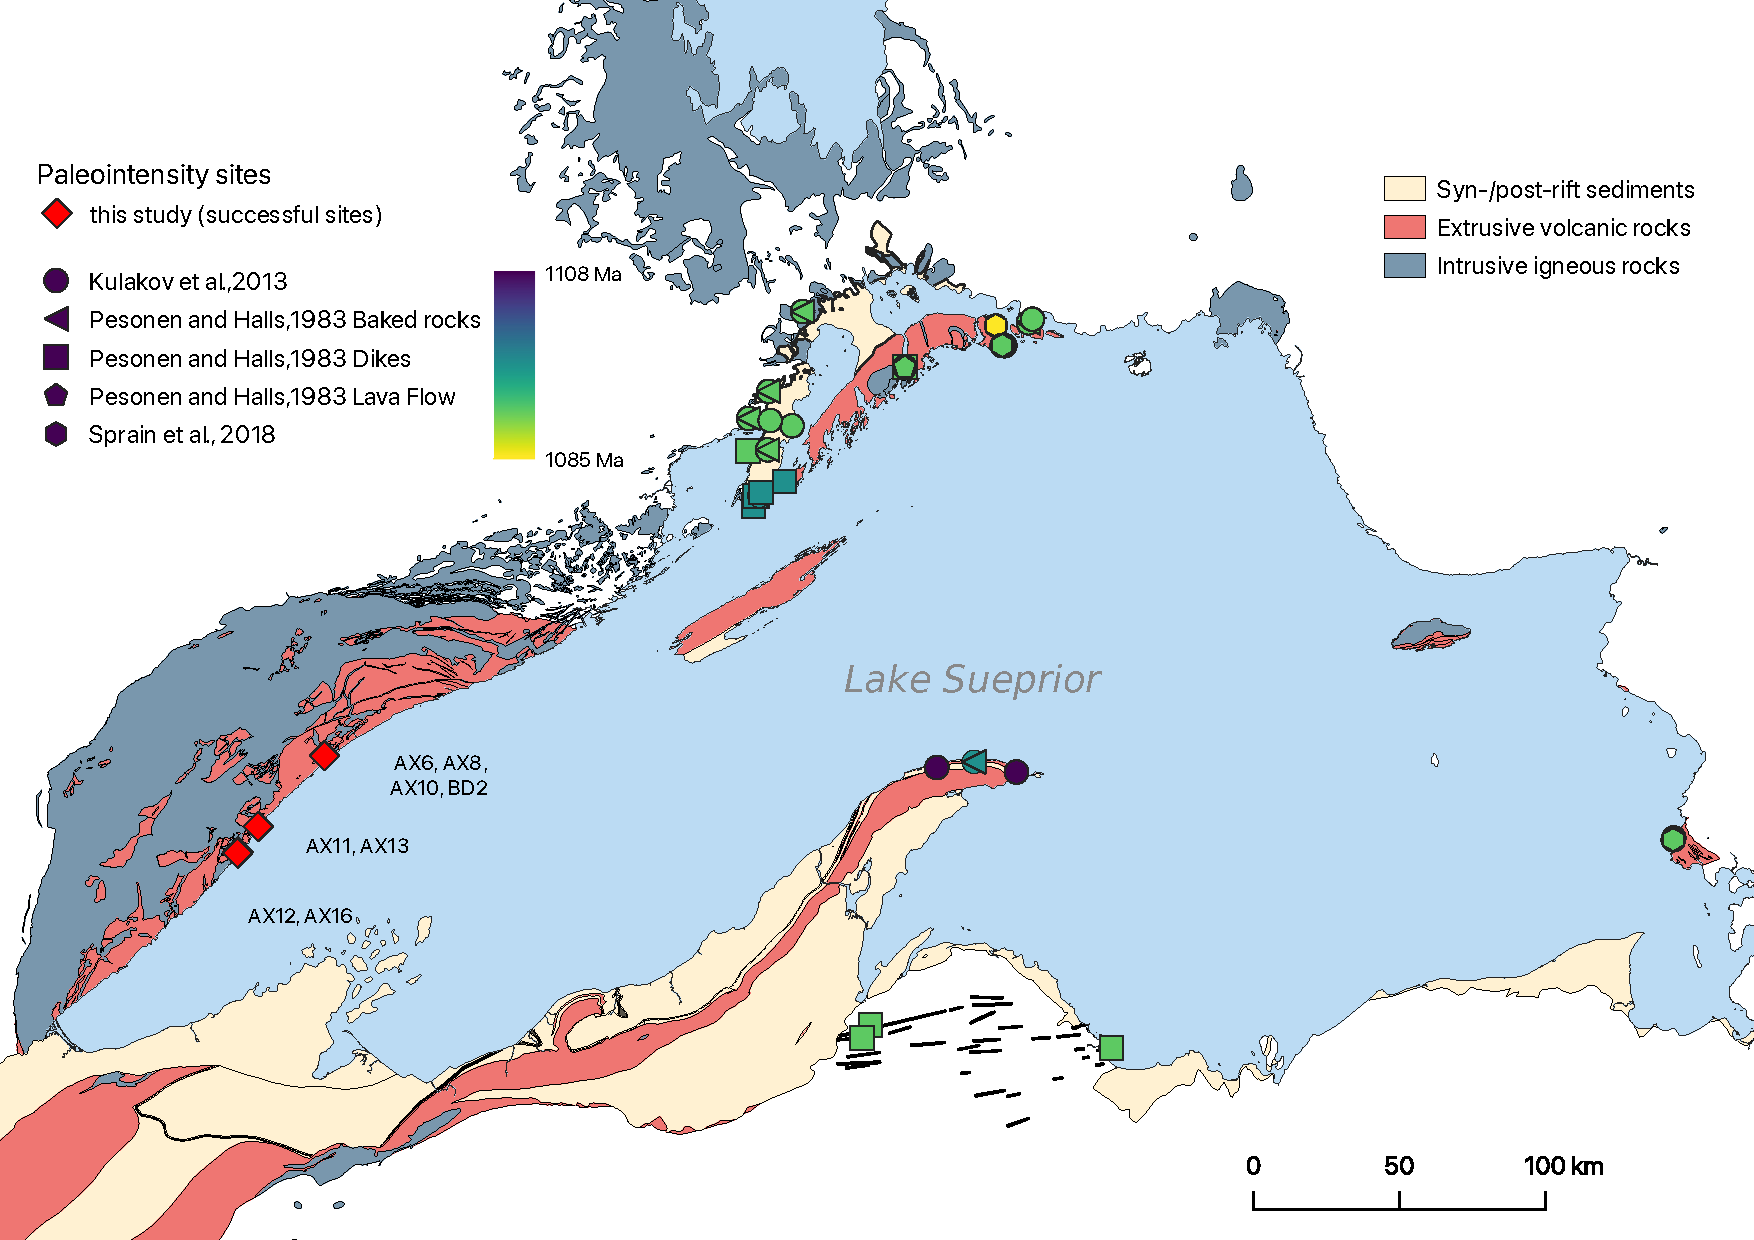
\includegraphics[width=4.75 in]{Geologic_map.pdf}
\caption{\footnotesize{}}
\label{fig:Geologic_map}
\end{figure}

The Beaver Bay Complex, which sits stratigraphically above the Duluth Complex, is another intrusive complex that resulted from main stage magmatism. The exposed area of the Beaver Bay Complex is $\sim$1000 km\textsuperscript{2} where it has been mapped along the northwestern shore of Lake Superior in northeastern Minnesota (Fig. \ref{fig:Geologic_map}). The Beaver Bay Complex is a multi-phase, composite intrusive complex that intrudes parts of the NSVG (Fig. \ref{fig:Geologic_map}; \citeA{Miller1997a, Swanson-Hysell2020a}). Distinct from the deep plutonic intrusions of the Duluth Complex, the majority of the Beaver Bay Complex is formed of hypabyssal intrusions that were emplaced as dikes and sills at shallow depths \cite{Miller1997a}. Most of the Beaver Bay Complex intrusions are dioritic to gabbroic in composition \cite{Miller1997a}. The main lithology of the Beaver River diabase dikes and sills network within the Beaver Bay Complex is an ophitic olivine gabbro (Fig. \ref{fig:Field_photo}), but in wider areas of dikes and the upper parts of thick sills, this rock type can abruptly transition into intergranular olivine oxide gabbro, then into subprismatic (and commonly foliated) ferrogabbro, and finally into granophyric monzodiorite. The more evolved and later emplaced components of the Beaver River diabase network are commonly distinguished as the Silver Bay intrusions in the southern Beaver Bay Complex (Fig. \ref{fig:Geologic_map}). Overall being intermediate in composition, the Silver Bay intrusions lithologies range from ophitic olivine gabbro to ferrogranite \cite{Shank1989a}. Field mapping by \citeA{Miller1994a} found intrusive relationships between the Silver Bay intrusions and the Beaver River diabase. Angular inclusions of the host Beaver River diabase within marginal zones of the Silver Bay intrusions led \citeA{Miller1997a} to interpret that the Silver Bay intrusions intruded after the diabase crystallized.

One distinctive feature of the Beaver River diabase is its inclusions of anorthosite xenoliths. In the southern part of the Beaver Bay Complex, the Beaver River diabase occurs as dikes and sills, typically including anorthosites with various sizes ranging from centimeters to over 150 meters (Figs. \ref{fig:Geologic_map}, \ref{fig:Field_photo}; \citeA{Grout1939a, Morrison1983a}). The diabase in this region intrudes the Palisade rhyolite of the North Shore Volcanic Group (Fig. \ref{fig:Geologic_map}), which has a $^{206}$Pb/$^{238}$U date of 1093.94 $\pm$ 0.28 Ma (2$\sigma$ analytical uncertainty is presented for CA-ID-TIMS dates throughout this work; \citeA{Swanson-Hysell2019a}). The Beaver River diabase is locally intruded by the Silver Bay intrusions (Fig. \ref{fig:Geologic_map}). An aplite unit within the granophyre zone of one of these Silver Bay intrusions has a $^{206}$Pb/$^{238}$U date of 1091.61 $\pm$ 0.14 Ma \cite{Swanson-Hysell2019a}. Another arcuate, sill-like diabase body mapped as the Beaver River diabase outcrops along the eastern part of the complex (Fig. \ref{fig:Geologic_map}; \citeA{Miller1997a}). The diabase composition there is similar to that in the south and it also contains large anorthosite xenoliths with dimensions that exceed 100 meters at Carlton Peak (Fig. \ref{fig:Geologic_map}). The Beaver River diabase in the northern part of the complex, near the Houghtaling Creek area, typically forms narrow, near-vertical dikes instead of sheets in the southern and eastern regions (Fig. \ref{fig:Geologic_map}; \citeA{Miller1994a}). The diabase in this region only locally contains xenoliths of anorthosite. 

Hundreds of anorthosite xenoliths have been recognized and mapped within the Beaver River diabase (Fig. \ref{fig:Geologic_map}). Many hill tops in the Beaver Bay Complex, such as Carlton Peak and Britton Peak, are large anorthosite blocks (which lead \citeA{Lawson1893a} to erroneously conclude that they were relict Archean topography). Later work established the anorthosite blocks as xenoliths, which are now extensively documented through geologic mapping of the region (Fig. \ref{fig:Geologic_map}; \citeA{Miller2001a, Miller1988a, Miller1989a, Boerboom2004a, Boerboom2006a, Boerboom2006b, Boerboom2007a}) and outcrop-scale exposures (Fig. \ref{fig:Field_photo}). In the field, the anorthosites typically appear as subrounded to rounded, light-colored, translucent blocks that are in sharp contact with the hosting diabase (Fig. \ref{fig:Field_photo}). They also occur as exposures whose contact with the diabase is covered (Fig. \ref{fig:Field_photo}). \citeA{Grout1939a} suggested that the rounded anorthosites are the result of abrasion during transportation as they were entrained by the diabase (i.e. physical weathering within a magmatic system). While the Beaver River diabase is chilled against the North Shore Volcanic Group lithologies that it intrudes, the diabase is not chilled against the margin of the anorthosite xenoliths \cite{Morrison1983a, Miller1997a}. The lack of chilled contacts is consistent with the anorthosite being at elevated temperatures and cooling at the same time as the diabase magma (Fig. \ref{fig:thermal_history_model}).

The anorthosite xenoliths are dominantly monomineralic plagioclase that has an average anorthite content of $\sim$70\% \cite{Morrison1983a, Doyle2016a}. Interstitial pyroxene and olivine are present in minor concentrations in the xenoliths. Within the Carlton Peak anorthosite xenolith, up to 10 cm oikocrysts of olivine and pyroxene can occur. Nevertheless, the overall olivine content in the anorthosites is low. Interstitial titanomagnetite-ilmenite intergrowths that exceed 100 $\mu$m can be found with microscopy and $<$20 $\mu$m Fe-Ti oxide grains can be detected with scanning electron microscopy (Fig. \ref{fig:Field_photo}). Based on textural differences \citeA{Morrison1983a} divided the anorthosite xenoliths into four groups: one group which typically have well-developed granoblastic texture characterized by equigranular plagioclase crystals; another group which have interlocking, lath-shaped plagioclase crystals; an intermediate group which can have both granoblastic texture and interlocking plagioclase laths; and a brecciated group that have brittle deformation textures superposed on pre-existing textures. 

The hypabyssal intrusions of the ophitic Beaver River diabase (BRD) and the Ca-rich anorthosite xenoliths that it hosts are the targets of this study. The diabase contains abundant Fe-Ti oxides which are dominant carriers of paleomagnetic information. The nearly-pure anorthosite xenoliths have potential for paleomagnetic investigation because plagioclase hosts can protect the exsolved magnetic minerals from post-formation alteration \citep{Tarduno2005a}, and thus may faithfully record paleointensity information at the time of formation. A typical outcrop of anorthosite xenolith residing in the diabase and a hand sample of the anorthosite are shown in Fig. \ref{fig:field}(A, B). Preliminary petrographic analyses show that the anorthosites are dominantly monomineralic with recrystallization textures (Fig. \ref{fig:field}C). Crosscutting relationships together with high-precision geochronology dates from \cite{Swanson-Hysell2019a} bracket the age of the BRD to be between 1091.61 $\pm$ 0.14 Ma  (the age of the younger Silver Bay intrusions) and 1093.94 $\pm$ 0.28 Ma  (the age of the Palisade rhyolite). 

High-precision $^{206}$Pb/$^{238}$U zircon date of 1091.83 $\pm$ 0.21 from one anorthosite in Silver Bay area tightly constraint the age of the diabase intrusion to be 1091.7 $\pm$ 0.2 Ma. previous paleomagnetic directional data from \citeA{Zhang2021a} reveal that vast majority of the anorthosite xenoliths have minimal secondary remanence and single component characteristic remanence magnetizations carried by low-Ti magnetite. Step-wise demagnetization experiments show that the characteristic remanence often unblock sharply between temperature steps 500\textdegree C and 580\textdegree C. Moreover, the site mean paleodirection of the anorthosite xenoliths share a common mean with the directions of their host diabase. Together with thermal conduction modeling, these data are consistent with the interpretation that the anorthosite xenoliths within the Beaver River diabase acquired remanence during cooling with the diabase after their hypabyssal emplacement. A total of  xxx specimens from xx sites were used for paleointensity experiments. The locations of the xx sites are shown in Fig. 1 and the corresponding site mean palaeomagnetic directions from \citeA{Zhang2021a} are shown in Fig. 2(b).







  
\begin{figure}
\noindent\includegraphics[width=\textwidth]{Field_photo_petro_photo.pdf}
\caption{\small{(A) A typical outcrop of an anorthosite xenolith residing in the Beaver River diabase. (B) A hand sample of anorthosite. The large reflective face at the bottom center is a cleavage plane of a centimeter-size plagioclase crystal. The scale is 9 cm in total. (C) Cross-polarized light image of an anorthosite thin section. The second order birefringence of plagioclase indicates a high Ca content. The closely packed plagioclase crystals show recrystallization texture. (D) High-magnification SEM image of Fe-Ti oxides exsolved from a pyroxene crystal included in a plagioclase crystal. (E) Large, interstitial magnetite-ilmenite intergrowths between two plagioclase crystals. (F) A large Fe-Ti oxide grain with magnetite-ilmenite intergrowths next to a pyroxene in diabase. an: anorthite; px: pyroxene; mag: magnetite; ilm: ilmenite}}
\label{fig:field}
\end{figure}

Most thermally demagnetized anorthosites and alternating field (AF) demagnetized diabase specimens have minimal secondary components and their magnetization is interpreted to be dominated by a primary thermal remanent magnetization. Characteristic magnetizations from both lithologies yield indistinguishable site-mean directions and the virtual geomagnetic poles (VGPs) fall close to the 1095 Ma pole from the synthesized APWP of \cite{Swanson-Hysell2019a}, which is in agreement with the geochronological constraints  (Fig. \ref{fig:pmag}). 

I conducted a comparative study of modified IZZI paleointensity experiments on both the diabase and anorthosite, with a group treated with low-field AF demagnetization after each in-field step and another group without. Paleointensity experiments for most diabase specimens result in non-ideal Arai plots often with poor pTRM checks, making them difficult to interpret for paleointensity estimate (Fig. \ref{fig:pmag}). These results can be interpreted to be associated with observed color change of the diabase after heating, which suggests alterations of the oxides. The experiments conducted on anorthosite samples, on the other hand, had a high success rate of $>$ 50\%. Moreover, the resulting success rate for the anorthosite group with the AF treatment is even higher. The more straight Arai plots are likely due to the AF steps mitigating the exhibition of pTRM tails often associated with non-ideal behavior of multi-domain grains that are demagnetized by the pre-treatment step. However, as the nearly pure anorthosite samples did not display dramatic alterations that are easily detectable with common petrographic techniques, a question rises as why some of the compositionally similar anorthosites passed the paleointensity selection results and some did not. 

\begin{figure}
\noindent\includegraphics[width=\textwidth]{pmag_plot_.pdf}
\caption{\small{(A) Site-mean directions of anorthosite and diabase plotted on an equal-area plot. (B) Calculated VGPs from the anorthosite and diabase plotted in context of a previously synthesized ca. 1.1 Ga Laurentia APWP from the Midcontinent Rift volcanics \citep{Swanson-Hysell2019a}. VGPs from both lithologies fall close to the 1095 Ma pole position. (C) Example Arai plots for diabase. Most diabase and many anorthosite specimens were rejected by selection criteria due to the zigzagging behavior shown in the diabase example plot. (D) Example Arai plots for anorthosite. A typical anorthosite specimen that passes selection shows straight Arai plot with a high paleointensity estimate before cooling rate correction. Note both specimens in (C) and (D) show dominantly single component magnetization in the inset orthogonal plots. The estimated field intensity is not cooling rate corrected.}}
\label{fig:pmag}
\end{figure}

At the IRM, I was seeking the answer to this question with the help of the vibrating sample magnetometer (VSM) systems, including a newly installed Lake Shore VSM which greatly helped improve measurement resolution on samples with weak magnetizations (Fig. \ref{fig:backfield}). Backfield demagnetization experiments were conducted and used to develop coercivity spectra (Fig. \ref{fig:backfield}). The spectra were subsequently modeled to fit for the distributions of different  populations of magnetic particles using similar procedure as \cite{Maxbauer2016a}. Most spectra can be well approximated with models with one component or two components with overlapping coercivity ranges (Fig. \ref{fig:backfield}). The dominance of single-component distributions from the unmixed coercivity spectra likely suggests minimal alterations or formation of secondary magnetic mineral within the samples. By compiling the values of median destructive field (MDF) from all measured specimens and categorizing them in terms of their sister specimens' paleointensity results, I found that the anorthosites samples that pass paleointensity selection criteria have distinctively higher MDF values than those did not (Fig. \ref{fig:backfield}), and all diabase specimens have low MDF values like the non-ideal anorthosites (Fig. \ref{fig:backfield}). The higher MDFs ($\sim$60 mT) of the anorthosites are similar to what is typical of stoichiometric, single-domain magnetite grains which are favored for paleointensity experiments. Furthermore, the low MDFs displayed in other specimens could be linked to a dominant population of large interstitial Fe-Ti oxides that are more likely to form multi-domain grains, which have been observed in both the anorthosite and diabase (Fig. \ref{fig:field}). In addition, preliminary tests on single anorthosite crystals might suggest that not all single crystals are necessarily better for paleointensity research when comparing to bulk samples, given their similar low MDF to the failed diabase and anorthosite specimens. However, more single crystal grains with paired paleointensity data and rock magnetic data may be needed before a general conclusion can be drawn. 

Taken together, the rock magnetism experiment results support my paleointensity selection criteria in that rock specimens that produce straight Arai plots and have MDF similar to stoichiometric single-domain magnetite are preferentially selected. The preliminary paleointensity results yielded consistent estimates. The cooling rate corrected site-mean paleointensity estimate is about 40 $\mu$T, consistent with results from \cite{Sprain2018a} that the Earth's magnetic field strength at surface in the late Mesoproterozoic was close to that of today. 

\begin{figure}
\begin{center}
	\noindent\includegraphics[width=0.5\textwidth]{backfield_example_.pdf}
\end{center}
\caption{\small{(A) Backfield measurement data acquired using a Princeton VSM on an anorthosite specimen. The noise level on coercivity plot is high and a heavy smoothing is needed to make subsequent coercivity modeling interpretable. (B) Backfield measurement data acquired using a Lake Shore VSM on the same specimen as that in (A). The inset coercivity unmixing plot shows that the much smoother initial backfield curve resulted in a tight single-component model fit. (C) Box plot of distribution of the median destructive field of all measured specimens. The anorthosite specimens that pass selection criteria have distinctly higher median destructive field (MDF) than other groups.}}
\label{fig:backfield}
\end{figure}










\section*{Method}
\subsection*{Sample collection}
Sample cores were collected using a hand-held drill and were ori- ented using a magnetic compass as well as a sun compass when possible. Palaeohorizontal was determined from intercalated sedi- mentary layers and flow tops. 6–10 cores were drilled from each lava flow in order to robustly determine an accurate site mean. More detailed information about the sites and their context along with directional results are reported in Swanson-Hysell et al. (2009, 2014a,b). For palaeointensity analysis, 5–8 samples per flow were chosen. Samples were chosen based on demagnetization behaviour with a preference for samples wherein relatively little remanence is held by haematite such that their magnetization is dominated by (titano)magnetite recording a primary thermal remanent mag- netization. Haematite can be a significant carrier of remanence in Mamainse Point basalts (see Swanson-Hysell et al. 2011) and other successions around the Midcontinent Rift. Given that haematite can form at the expense of magmatic (titano)magnetite, such flows were deemed to not be appropriate targets for the palaeointensity experiments.

\subsection*{Paleointensity experiment}
A total of 133 specimens from 21 selected sites underwent palaeoin- tensity experiments that followed the stepwise double-heating Thel- lier method (Thellier & Thellier 1959), using the IZZI protocol (Tauxe & Staudigel 2004). pTRM checks were performed systemati- cally throughout the experiment to test whether there was significant mineralogical alteration due to heating and were assessed using the SCAT parameter of Shaar & Tauxe (2013). All remanence measure- ments were made on a 2G Enterprises DC-SQUID superconduct- ing rock magnetometer equipped with an automated pick-and-place sample changer system at the UC Berkeley Paleomagnetism labora- tory. The magnetometer is housed inside a three-layer magnetostatic shield that maintains background fields of less than 500 nT. Heating steps were performed using an ASC TD-48SC thermal demagne- tizer with a controlled field coil that allows for a magnetic field to be generated in the oven in conjunction with a DC power sup-ply. The thermal demagnetizer was degaussed with an alternating field following ‘in-field’ steps such that residual fields were <10 nT during ‘zero-field’ steps. Samples were placed in the same location within the thermal demagnetizer for each heating step and were maintained in the same orientation with regard to the applied field. During each heating step, samples remained at peak temperatures for 20 min. An applied laboratory field of 30 μT was used for all in- field steps. All heating steps were performed in air. The temperature increments for the experiments were chosen to cover characteristic remanent magnetizations held by (titano)magnetite, with smaller increment temperature steps performed close to the expected un- blocking temperature of stoichiometric magnetite. Hysteresis mea- surements were conducted at the Institute for Rock Magnetism at the University of Minnesota. Major hysteresis loops were mea- sured at room temperature using a Micromag Princeton Measure- ments vibrating sample magnetometer with nominal sensitivity of 5 × 10−9 Am2.

A total of 59 specimens from 13 anorthosite sites and 46 specimens from 7 diabase sites underwent paleointensity experiments that followed the stepwise double-heating Thellier method with temperature steps up to 585 $^\circ$C \cite{Thellier1959a, Tauxe2004a}. On top of the IZZI modification of the Thellier experimental protocol, we also performed a comparative study where we added an extra step of 20 mT alternating field (AF) cleaning on half of the specimens after each in-field step. The purpose is to study whether the AF step could help improve specimens' behavior during paleointensity experiments. pTRM checks were performed systematically throughout the experiment to test whether there was significant mineralogical alteration due to heating and were assessed using the SCAT parameter of \citeA{Shaar2013a}. All remanence measurements were made on a 2G Enterprises DC-SQUID superconducting rock magnetometer equipped with an automated sample changer system in the paleomagnetism lab at UC Berkeley. Heating steps were performed using an ASC TD-48SC thermal demagnetizer with a controlled field coil that allows for a magnetic field to be generated in the oven in conjunction with a DC power supply. The thermal demagnetizer was degaussed with an alternating field following in-field steps such that residual fields were $<$10 nT during zero-field steps. Samples were placed in the same location within the thermal demagnetizer for each heating step and were maintained in the same orientation with regard to the applied field. During each heating step, samples remained at peak temperatures for 20 min. An applied laboratory field of 30 $\mu$T was used for all in-field steps. All heating steps were performed in air. The temperature increments for the experiments were chosen to cover characteristic remanent magnetizations held by (titano)magnetite, with smaller increment temperature steps performed close to the expected unblocking temperature of stoichiometric magnetite. 



\subsection*{Paleointensity result selection}
The following criteria were used as quality filters on the palaeoin- tensity results: (1) a maximum angular deviation (MAD; Kirschvink 1980) of <20◦; (2) scatter parameter (β; Coe et al. 1978) values of <15 per cent; (3) a deviation angle (DANG; Tanaka & Kobayashi 2003; Tauxe & Staudigel 2004) of < 5◦; (4) fraction of remanence (FRAC; Shaar & Tauxe 2013) >0.6; (5) scatter statistic (SCAT; Shaar & Tauxe 2013) = TRUE; (6) a maximum gap (GAP-Max; Shaar & Tauxe 2013) < 0.6; (7) number of pTRM checks > 2; (7) and number of measurements used for palaeointensity determi- nation ≥ 4; (Table 1)

The following criteria were used as quality filters on the paleointensity results: (1) a maximum angular deviation (MAD; \citeA{Kirschvink1980a}) of $<$ 20; (2) scatter parameter ($\beta$; citeA{Coe1978a}) values of $<$ 15 \%; (3) a deviation angle (DANG; \citeA{Tanaka2003a}; \citeA{Tauxe2004a} of $<$ 5; (4) fraction of remanence (FRAC; \citeA{Shaar2013a}) $>$ 0.6; (5) scatter statistic (SCAT; \citeA{Shaar2013a}) = TRUE; (6) a maximum gap (GAP-Max; \citeA{Shaar2013a}) $<$ 0.6; (7) number of pTRM checks $>$ 2; (7) and number of measurements used for paleointensity determination $\geq$ 4; (Table \ref{tab:criteria}). The MAD measures the scatter about the best-fit line through NRM steps in the selected interval for which the intensity is defined. DANG, the deviation angle, is the angle between the best-fit direction that is free floating and the direction between the centre of mass of the data and the origin of the vector component diagram (\citeA{Tanaka2003a}; \citeA{Tauxe2004a}). Both MAD and DANG assess the directional variation of the NRM, with MAD measuring the scatter in the NRM directions and DANG assessing whether the component is trending toward the origin of the Zijderveld plot. $\beta$ is the ``scatter" parameter of \citeA{Coe1978a} and is the ratio of the standard error of the slope of the best-fit line of the selected NRM and pTRM points on an Arai plot to the absolute value of the slope. FRAC is the fraction of the NRM that is used in the best-fit line \cite{Shaar2013a}. The FRAC value was chosen to preferentially select samples with dominantly single-slope Arai plots. GAP-Max is the maximum gap between two points on the Arai plot determined by vector arithmetic. SCAT is a Boolean operator which uses the error on the best-fit slope of the selected data on the Arai plot to determine if the data are overly scattered. The parameter is used to assess pTRM checks in addition to assessing the degree to which IZZI steps are zigzagged. $\beta$, FRAC, GAP-Max and SCAT are all statistics to assess the behavior of Arai plots. See the Standard Paleointensity Definitions (\citeA{Paterson2014a}, https://earthref.org/PmagPy/SPD/home.html, last accessed 2018 March 17) for more details. Data analysis was conducted using Thellier GUI \cite{Shaar2013a} within the PmagPy software package \cite{Tauxe2016a}. 


\subsection*{Rock magnetic experiment}

Hysteresis, backfield, and magnetic property measurements were conducted at the Institute for Rock Magnetism (IRM) at the University of Minnesota. Major hysteresis loops and backfield curves were measured at room temperature using a Micromag Princeton Measurements vibrating sample magnetometer with nominal sensitivity of $5 \times 10^{-9}$ Am\textsuperscript{2}. We used the magnetic property measurement system (MPMS) at the IRM to aid in the identification of magnetic mineral. The operational sequence follows an in-field cooling step in a 2.5 T field from room temperature to 10 K, a zero-field cooling from room temperature to 10 K, and a final cooling from room temperature to 10 K after an IRM acquisition at room temperature. 

Backfield demagnetization experiments were conducted and used to develop coercivity spectra (Fig. \ref{fig:backfield}). The spectra were subsequently modeled to fit for the distributions of different  populations of magnetic particles using similar procedure as \cite{Maxbauer2016a}. Most spectra can be well approximated with models with one component or two components with overlapping coercivity ranges (Fig. \ref{fig:backfield}). The dominance of single-component distributions from the unmixed coercivity spectra likely suggests minimal alterations or formation of secondary magnetic mineral within the samples. By compiling the values of median destructive field (MDF) from all measured specimens and categorizing them in terms of their sister specimens' paleointensity results, I found that the anorthosites samples that pass paleointensity selection criteria have distinctively higher MDF values than those did not (Fig. \ref{fig:backfield}), and all diabase specimens have low MDF values like the non-ideal anorthosites (Fig. \ref{fig:backfield}). The higher MDFs ($\sim$60 mT) of the anorthosites are similar to what is typical of stoichiometric, single-domain magnetite grains which are favored for paleointensity experiments. Furthermore, the low MDFs displayed in other specimens could be linked to a dominant population of large interstitial Fe-Ti oxides that are more likely to form multi-domain grains, which have been observed in both the anorthosite and diabase (Fig. \ref{fig:field}). In addition, preliminary tests on single anorthosite crystals might suggest that not all single crystals are necessarily better for paleointensity research when comparing to bulk samples, given their similar low MDF to the failed diabase and anorthosite specimens. However, more single crystal grains with paired paleointensity data and rock magnetic data may be needed before a general conclusion can be drawn. 

\section*{Results and Discussion}
\subsection*{Paleomagnetism}
The paleodirectional results of AF demagnetization of 7 diabase sites and thermal demagnetization of 16 anorthosite sites are shown in Table \ref{tab:}. In some cases, specimens from both lithologies show a minimal remanence component that was removed during very low AF field ($<$ 10 mT) for diabase and during low temperature demagnetization steps for anorthosites ($<$ 300 $^\circ$C). This component is likely a modern day field overprint, since its direction resembles the present-day field direction. The dominant components in both lithologies are northwest and down (Figure \ref{fig:directions}). This is likely the primary remanent magnetization recorded by the diabase and anorthosite during the emplacement of the diabase, since it is origin-trending and the principal component fitting yielded good specimen-level and site-level consistence. Common mean test (\cite{McFadden1990a}) results based on site-level directional comparison between anorthosites and their in situ diabase hosts are shown in Figure \ref{fig:directions}. Most anorthosite-diabase pairs have tightly clustered directions, and the three anorthosite sites that do no pass the statistical test with their diabase hosts nevertheless have within-site coherent directions that are close to the diabase directions (Figure \ref{fig:directions}). Putting the grand mean paleodirections and inferred virtual geomagnetic poles (VGPs) of both lithologies together in context of a previously synthesized apparent polar wander path (APWP) from the volcanics of the Midcontinent Rift \cite{Swanson-Hysell2019a}, we find the pole positions recovered from both the diabase and anorthosite to be lying close to the estimated VGP position around 1095 Ma, which is consistent with the geochronology constraints (between 1093.94 $\pm$ 0.28 Ma and 1091.61$\pm$ 0.14 Ma, \cite{Swanson-Hysell2019a}). 

Paleointensity experiment results show three types of dominant specimen behaviors on Arai plots (Figure \ref{fig:Arai_plot}): dominantly single-slope (--- out of --- specimens), double- slope (--- out of --- specimens) and zigzagging (--- out of --- specimens) (Figure \ref{fig:Arai_plot}). It is worth mentioning that almost all specimens have single direction demagnetization result as in Zijderveld plots of all zero-field steps. Upon applying the paleointensity result selection criteria (Table \ref{tab:}), we found a total of 31 out 59 anorthosite specimens and 4 out of 46 diabase specimens were accepted, yielding 7 anorthosite sites and 1 diabase sites with interpretable site-level paleointensity results (Table \ref{}). The selection criteria successfully rejected double-slope results (FRAC $>$ 0.6) and zigzagging results ($\beta$, DANG, and SCAT parameter). In addition, some rejected specimens have poor pTRM checks especially at high temperature steps (Figure \ref{fig:Arai_plot}). This may suggest a high degree of alteration in magnetic mineralogy during heating steps. The accepted anorthosite specimens do display straight Arai plots and the accepted fractions of temperature steps are mostly covering the primary remanence components (Figure \ref{fig:Arai_plot}). In terms of the diabase specimens, all but four of them failed the selection because double-sloping Arai plots, poor pTRM checks, and zigzagging behaviors (Figure \ref{fig:Arai_plot}). Even specimens in site BD2, the only site that passed selection, do not always display ideal Arai plots (Figure \ref{fig:Arai_plot}). Additionally, all accepted results from site BD2 are from low-temperature fractions of Arai plots (below 500 $^\circ$C), which are different than those used in anorthosite sites (typically above 500 $^\circ$). Although the lower temperature fraction of the Arai plots are straight and pTRM checks are consistent (Figure \ref{fig:Arai_plot}), we have to acknowledge the existence of second slopes at high temperature fractions (Figure \ref{fig:Arai_plot}). Nevertheless, the interpreted ancient geomagnetic field value from the accepted slopes is very similar to those reported by anorthosites (Figure \ref{fig:Arai_plot}). 

In this study, it is particularly important to assess the cooling rate effects, remanence anisotropy, and potential non-linear TRM or pTRM acquisition characteristics of diabase and anorthosites. Because the cooling duration of intrusive rocks could be much longer than the extrusive rocks, the slowly cooled diabase and anorthosite can bias laboratory paleointensity estimates toward an overestimate for SD grains \cite{Dodson1980a, Halgedahl1980a, Selkin2000a} or underestimation for MD grains \cite{McClelland-Brown1984a}. Further, preferred orientations of ferromagnetic fabrics along plagioclase crystallographic orientations in anorthosites could introduce a large degree of anisotropy in remanent magnetizations \cite{Selkin2007a, Biedermann2018a}. \citeA{Selkin2007a} reported that large, acicular SD grains can have profound non-linear acquisitions of TRM. According to their experiments, grains with such characteristics that are hosted within silicate crystals can saturate in fields as low as earth's field \cite{Selkin2007a}. 

Backfield experiment results suggest that the dominant remanence carrier in accepted anorthosite sites are likely SD magnetite (Figure \ref{fig:MDF}). The median destructive fields (MDF) of all accepted anorthosites are distinctively higher than those of the rejected anorthosites and the diabase. Moreover, the median of the MDFs of accepted anorthosites is about 50 mT, which is in the expected range of typical no-interactive SD magnetite grains. In addition, the anorthosites' narrow unblocking temperatures near the magnetite curie temperature also support that we idealize the remanence carriers in anorthosites to be SD magnetite. 

From the thermal history model we can also estimate the time duration which the diabase and anorthosite spent to block in the primary component of their remanence. We found the cooling time to be on the order of magnitude of $\sim$1 kyr from 580 to 500 $^\circ$C, which corresponds to a cooling rate of $1.6\times10^{-9}$ $^\circ$C s$^{-1}$. In contrast, the lab cooling rate is much faster, at about $1.3\times10^{-1}$ $^\circ$C s$^{-1}$ if we assume it takes 10 minutes in lab condition to cool through the same temperature interval. As a result, this significant cooling rate difference leads to a prediction of 35.5\% overestimate of true field \cite{Halgedahl1980a}. We therefore correct our paleointensity results by a factor of 0.74. 

It has been well illustrated through experiments on anorthosites that anisotropic remanence acquisition can have a significant impact on paleointensity estimates \cite{Selkin2000a}. Following similar experiment protocol, we found that at least the bulk anorthosite specimens in this study are not very anisotropic. This result can be further supported by the fact that the recovered paleodirectional data from the anorthosite closely match those from the paired diabase hosts (Figure \ref{fig:directions}), the lithology of which is usually considered isotropic in terms of recording remanence magnetization. Both the diabase and anorthosite display consistent interpreted VGPs at the time of emplacement that matche with the expected position based on the volcanic APWP record (Figure \ref{fig:poles}, \citeA{Swanson-Hysell2019a}). We therefore do not correct our samples for anisotropy of remanence. 

We also performed non-linear full TRM checks following the experiment protocol proposed by \citeA{Selkin2007a}. We imparted full TRMs on our anorthosite specimens (after the paleointensity experiment) by heating them up to 600 $^\circ$C and cooling in field of 30, 50, 70, and 90 $\mu$T respectively. Unlike the anorthosites studied by \citeA{Selkin2007a}, none of our specimens show a saturating trend at progressively higher fields. More, the normalized magnetizations show nearly linear relationship with lab field strengths. There is thus no need for correcting non-linear thermal remanence acquisitions. 

Figure \ref{fig:PINT_plot} shows all accepted anorthosite and diabase specimen paleointensity results and their site-level means with one standard deviation envelopes. An anorthosite site mean paleointensity weighted by site standard deviations is plotted as a dashed orange line, and the standard deviation envelope as dashed green lines. The anorthosites are also grouped by their geographical vicinities \ref{fig:PINT_plot}. The site-level results are shown in Table \ref{tab:PINT_result}. Anorthosite sites AX10, 11, 12, 13, 16 yielded very high within-site coherence (Figure \ref{fig:Arai_plots, fig:PINT_plot}), which suggest high-confidence site-level paleointensity estimates. Clearly there are two populations of paleointensity results: a group of high estimates from anorthosite site 11 and 13 which have very high within-site consistency and are in agreement with the results from BRD site 2; and another group of low estimates from anorthosite site 6, 8, 10, 12, and 16, which also have tight agreement across sites.

\subsection*{Rock magnetism}
\begin{figure}[h!]
\noindent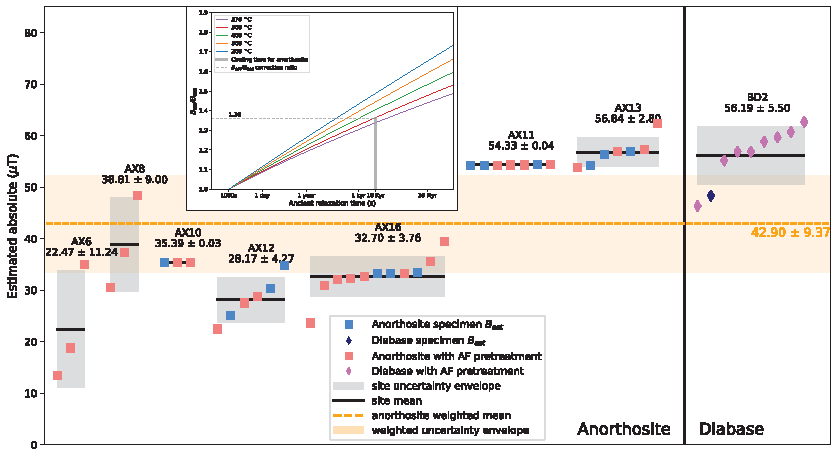
\includegraphics[width=0.5\textwidth]{manuscript/Paleointensity_plot_cooling_corrected.pdf}
\centering
\caption{\small{ }}
\label{fig:PINT_cooling_corrected}
\end{figure}



% that this study has robust data, discuss the reasoning using rock mag data that reflect the success and failure in PINT experiment


% cooling rate correction problem - that the Nagy et al paper can suggest even less of a correction and higher of the estimated field. theoretical thermal modeling by \citeA{Zhang2021a} suggest tha the anorthosite xenoliths were likely heated to diabase magma temperature regardless of their sizes, and cooled through the typical characteristic unblocking temperature range from 580 to 500 on the order of 1000 years. Comparing to the typical lab cooling time of about 100 seconds duirng paleointensity experiments, the significantly slower cooling rate when the NRM was acquired as the anorthosite xenoliths cooled with the diabase led to overestimate of paleointensity by up to 40\%. Overall range of correction factor can be 1.1-1.4, in any case consistent with a high field strength


% that this dataset also could have suffered from problem of averaging out secular variations, given that the mean pmag directions deviate from what is expected from the sythesized APWP, nevertheless the variations in estimate absolute paleointensity lead us to interpret that albeit close, the they intensity data were acquired at distinctly different times that are sufficiently far apart such that the surface geomagnetic field had already changed. 

% that \citeA{bono2019a} proposed an interesting trend but has problems in the directions, likely to be a short term feature of a low field during a reversal, instead of a low field as a result of long term cooling. 

% that Lloyd 2021 also presented low field that fits the trend, but they similarly have the issue of reversal, and that they do not have good control on secular variations

% Together with previously published data, the Midcontinent Rift rocks are recording 1.1 Ga earth geomagnetic field that is stronger than the mean of the past 300 Ma (Fig. \ref{}). 




\section*{Conclusion}
high success rate comparing to volcanics (more than half success sites), producing good consistent site level results, and across sites report present-day like field like today.

AF pre-treatment is helpful in that it increase the specimens/sites passing the selecting criteria, suggesting that the method likely helped improve the MD ferromagnetic carriers. 

Rock mag and petrographic data might suggest differences in terms of the value of peak field on coercivity spectra between those passed and those didn't.  

IRM measured before and after an acid dunk in --- concentration acid on specimens after IZZI experiment show a difference (significant drop) maybe? between specs that passed and those did not.

geographical association

Anyways. anisotropy of full TRM experiment on accepted specs show low degree of bulk sample scale full TRM anisotropy, with a range of ---. Cooling rate correction based on \cite{Halgedahl1980a} suggest a lab over estimate of B ancient of 35 \%, assuming constant cooling rate in natural condition. The cooling rate corrected field is $\sim$40 $\mu$T which is similar to today's field strength at similar latitude. 

\acknowledgments
Project research was supported by NSF CAREER grant EAR-1847277 to N.L.S.-H. and an Institute on Lake Superior Geology Student Research Fund grant to Y.Z. Permits for fieldwork and sampling from the Minnesota Department of Natural Resources are gratefully acknowledged. We thank James Pierce for assistance in the field.
We thank Dario Bilardello, Peat Solheid, Mike Jackson, Josh Feinberg, and Bruce Moskowitz for their tremendous help of instrumental operations, data interpretations, and research guidance. Y.Z. thanks the IRM for the U.S. Visiting Student Fellowship. Paleomagnetic data associated with this study are available within the MagIC database (\url{}; UPDATE WHEN DOI IS GENERATED) and all data are within a Github repository associated with this work (\url{}) that is also archived on Zenodo (INSERT URL AT TIME OF PROOFS). This repository also contains Python code related to calculations, visualizations and statistical tests discussed herein.  

\bibliography{YZ_ref}


\end{document}


% potential reviewer: Peter Selkin, Jeff Gee, Lisa Tauxe, Roger Fu, Lauri Pesonen, Josh Feinberg Julie Bowles, 



